% !TEX program = xelatex

\documentclass[10pt,a4paper,twocolumn]{article}
\usepackage{fontspec}
\setmainfont{Times New Roman}
\setmonofont{Menlo}
\usepackage{ctex}
%\usepackage{times}
\usepackage{geometry}
\geometry{left=20mm,right=20mm,top=1.3in,bottom=1.5in}

\usepackage{amsmath,amssymb,amsthm}

\usepackage{graphicx}
\usepackage{fancyhdr}

\usepackage{fancyhdr}
\usepackage{graphicx}
\usepackage{titlesec}
\usepackage{titletoc}
\usepackage{listings}
\usepackage{appendix}
\usepackage{bm}
\usepackage{amsmath}
\usepackage{amsfonts}
\usepackage{amssymb}
\usepackage{amsthm}
\usepackage{multirow}
\usepackage{subfig}
\usepackage{url}
\usepackage[style=gb7714-2015]{biblatex}
\usepackage{array}
\usepackage{booktabs}
\usepackage{multicol}
\usepackage{cuted}
\usepackage{stfloats}
\usepackage{lipsum}
\usepackage{indentfirst}
\usepackage{setspace}
\usepackage{enumerate}
\usepackage{enumitem}
\usepackage{footnote}
\usepackage{tabularx}
\usepackage{calc}
\usepackage{flushend}
\usepackage{sectsty}
\allsectionsfont{\heiti}
\usepackage{listings}
\usepackage[dvipnames]{xcolor}
\definecolor{dkgreen}{rgb}{0,0.5,0}
\definecolor{gray}{rgb}{0.5,0.5,0.5}
\definecolor{mauve}{rgb}{0.58,0,0.82}
\lstset{
  numbers=none,  
  frame=tb,
  aboveskip=3mm,
  belowskip=3mm,
  showstringspaces=false,
  columns=fixed,
  framerule=1pt,
  rulecolor=\color{gray!35},
  backgroundcolor=\color{gray!5},
  basicstyle={\ttfamily\scriptsize},
  numberstyle=\tiny\color{gray},
  keywordstyle=\color{blue},
  commentstyle=\color{dkgreen},
  stringstyle=\color{mauve},
  breaklines=true,
  breakatwhitespace=true,
  tabsize=2,
  extendedchars=false,
  postbreak=\mbox{\hspace{-4.9mm}\textcolor{purple}{$\hookrightarrow$}\space},
  caption={\protect\filename@parse{\lstname}\protect\filename@base\text{.}\protect\filename@ext},
  morekeywords={Title,Style,Flats,Sharps,Bars,Line,Meter,Size,Width}
}
\renewcommand{\lstlistingname}{代码}
\usepackage[hidelinks]{hyperref}
\addbibresource{reference.bib}

% \renewcommand{\kaishu}{\itshape}
% \renewcommand{\heiti}{\bfseries}
% \renewcommand{\fangsong}{\scshape}

%\mtxlatex

\title
{
  {\Huge\heiti\bfseries 瓦格纳歌剧与社会}\\
  {\fangsong \Large ——以马克思主义分析瓦格纳歌剧艺术与社会存在的辩证关系}
}
\author
{
  \Large 61520522 赵舞穹\thanks{邮箱:\href{mailto:wqzhao@seu.edu.cn}{wqzhao@seu.edu.cn},提交日期:\today{}。此报告的部分内容在课堂上进行了口头分享。}\\
  \\
  \normalsize{东南大学吴健雄学院 615205 班}\\
  \normalsize{中国南京 211189}
}
\date{\nonumber}

\pagestyle{fancy}
\fancyhf{}
\cfoot{\thepage}
\chead{瓦格纳歌剧与社会——以马克思主义分析瓦格纳歌剧艺术与社会存在的辩证关系\; {\kaishu 赵舞穹}}

\begin{document}

  \maketitle
  \begin{strip}
    {
      \centering
      \textbf{\heiti\large 摘要}

      ~

      \hspace*{\widthof{泰迪}}
      瓦格纳的歌剧在整个音乐和艺术的历史上留下了浓墨重彩的一笔。
      作为歌剧和音乐形式的伟大变革,他的作品影响力超越了艺术的范畴,
      从一个高层次反映了社会现实,也影响着后续社会的发展。
      瓦格纳歌剧作为德国艺术的典型代表之一象征了社会存在的一个维度,
      与社会存在有着辩证的关系。
      从瓦格纳歌剧的表现形式和内在哲学价值的基础上,
      本文分析了其体现的社会存在和社会意识辩证关系,
      并对其现代意义给出了阐释。
    }
    \\

    \textbf{\heiti 关键词:\ } {\kaishu 歌剧艺术\; 瓦格纳\; 马克思主义哲学\; 社会存在\; 社会意识}\\
  \end{strip}

  \section{瓦格纳歌剧艺术}

    谈到歌剧艺术,大家首先会想到意大利的歌剧或法国的大歌剧(grand opera)。
    不过在德国(Deutschland)
    这个有着深厚哲学基础的国家,
    开创出了 Musikdrama 这种独特的歌剧艺术形式。
    德语 Musikdrama 对应英文的 music drama,即音乐戏剧\cite{vernon2021disturbing}。
    创造出这种划时代艺术形式的作曲家就是瓦格纳(Richard Wagner)。
    
    对于瓦格纳,他的歌剧不再是一种娱乐的媒介,
    而成为了一种具有哲学意义的艺术形式。
    歌剧不再是歌唱演员秀歌喉而乐团辅助的场合,
    而是歌手和乐团一同营造歌剧的超强戏剧性。
    在瓦格纳歌剧中,歌手往往需要用极大的声音与乐团抗衡,
    将情感表现地淋漓尽致。
    具体来说,
    他大量运用了主导动机(Leitmotiv),为歌剧带来了全新的听觉体验。
    图~\ref{fig:hero} 中即是他最长的歌剧系列《尼伯龙根的指环》(Der Ring des Nibelungen)中的第三天《诸神的黄昏》(Götterdämmerung, 1876)中英雄齐格弗里德(Siegfried)的主导动机。
    \begin{figure}[htbp]
      \centering
      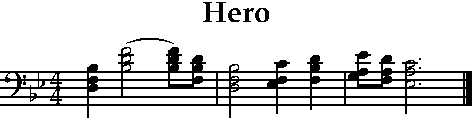
\includegraphics{music/hero-crop.pdf}
      \caption{英雄的主导动机\cite{wagner1876gotterdammerung}}
      \label{fig:hero}
    \end{figure}

    看到这样的音乐结构的第一感受就是其复杂性。
    瓦格纳的歌剧不再是简单的音乐线条,
    而是复杂的具有丰富细节的音乐,
    有着极强的张力。

  \section{社会存在与社会意识}

    瓦格纳的歌剧艺术产生自其特殊的社会时代,
    是由社会存在所决定的。
    不过,他的歌剧作品对之后的社会产生了深远影响,
    也反作用于社会意识。
    在第~\ref{sec:details} 节探讨具体的辩证关系之前,
    此处首先介绍社会存在和社会意识到基本概念。

    \subsection{社会存在}

      ``社会存在是指社会物质生活条件,是社会生活的物质方面,主要包括
      自然地理环境、人口因素和物质生产方式。''\cite{book}
      对于瓦格纳,他所处的德意志神圣罗马帝国末期诸侯割据的背景则是大的社会存在背景。

    \subsection{社会意识}

      ``社会意识是社会存在的反映,是社会生活的精神方面。''\cite{book}
      其中意识形态包括了政治法律思想、道德、艺术、宗教、哲学等。
      与之相对的,自然科学等则是非意识形态。

      艺术是社会意识的重要组成部分,
      ``艺术是通过塑造具体生动的形象来反映社会生活的意识形式。''\cite{book}
      很多时候,我们去了解一个社会的意识形态,
      也都是从艺术这个角度来切入的。

  \section{瓦格纳歌剧的四重境界}\label{sec:details}

    社会意识和社会存在互相都有着作用,
    这种相互作用的关系在深度学习(deep learning)中也有着其应用,
    例如强化学习(reinforcement learning)中智能体(agent)与环境(environment)
    有着互相反馈的过程。
    因此,我总结瓦格纳歌剧为四重境界,并从中分析艺术这种社会意识与社会存在的辩证关系。

    \subsection{个人理想}

      瓦格纳的歌剧往往都较为深刻,其传达表现的意识往往都会超过个人理想这个层次,
      不过在部分作品中的表现还是相对较为明显,反映的也是对应的社会存在。

      他早期的歌剧《漂泊的荷兰人》(Der fliegende Holländer, 1843)
      有很多片段中描述了他在海上流亡的生活,
      正如神话中漂泊的荷兰人一样经历困苦的生活。
      海上漂泊时水手的歌谣也被他选取提炼进入了歌剧。
      歌剧中体现的为生命存活挣扎的原始激情即是动荡社会的意识表现。
      这里存在一个非常值得探讨的问题是社会意识与个人意识的关系。
      因为个人所处的环境(即社会存在)有一定的相似性,因此个人的意识往往在一定程度上可以反映对应的社会意识,
      或者被社会所接受或诠释为其意识形态。
      正因此,个人创作的艺术作品在一些时候可以被认为是社会意识。
      不过当社会基础发生变化,这样的关系可能就不成立了。
      例如他的《唐豪瑟与瓦特堡歌唱大赛》(Tannhäuser und der Sängerkrieg auf Wartburg, 1845)
      于 1861 年在法国巴黎首演失败,他说``法国人无法欣赏德意志艺术'',
      在一个方面反映的就是不同的社会存在下欣赏艺术这种社会意识体现的结果是不一样的,
      当社会意识与社会存在存在某种强烈的耦合时这种共鸣才会达到最强烈的效果。

    \subsection{国家情怀}

      音乐家往往都有着自己的政治抱负,瓦格纳也不例外,
      刚在位于德累斯顿(Dresden)的宫廷剧院获得乐长职务小获成功,
      就参与了德累斯顿革命,为统一的德国而争斗。
      瓦格纳自己对社会的进步发展有着极大的期望,尤其是因为在他所处的年代,统一的德国还没有形成,
      四分五裂的政治格局让他对于国家统一和强大有着很强的信念\cite{vernon2021disturbing}。
      《黎恩济,最后的护民官》(Rienzi, der Letzte der Tribunen, 1842)
      中描述了罗马护民官为人民争取自由的失败尝试;
      《罗恩格林》(Lohengrin, 1850)中强调纯粹的德国不受到巫术的侵蚀,
      圣杯(Heiliger Gral)派遣圣杯骑士罗恩格林保卫;
      最重要的一部体现国家情怀的作品《纽伦堡的名歌手》(Die Meistersinger von Nürnberg, 1868)
      叙事角度却不同,他描述了德国中部纯粹的城市纽伦堡的市民阶级,
      ``德国人民爱艺术'',
      名歌手(Meistersinger)们将原汁原味的德意志艺术传递给人民。
      这里还强调了只有坚持对纯粹的艺术的热爱而提防外来民族的危机。

      在这样的三部作品中,体现的都是瓦格纳的国家情怀。
      前两部都是古时强大的统一时代,与真实的社会存在不同,
      ``进步的社会意识可以在一定程度上预见、推断未来,指导人们的实践活动''\cite{book},
      这种具有国家情怀的愿景即是这样的意识。

      《纽伦堡的名歌手》从一个小的角度即可以调动民族的认同,
      是瓦格纳透过了分裂的国家看到足以维系国家的共通之处,
      因此是如此令人感动。
      也是因为类似的原因,希特勒(Adolf Hitler)经常采用这部作品用作政治宣传。
      现在许多人以此认为瓦格纳的歌剧作品传达错误的观念,
      这其实是不客观的。
      正如我之前所说,艺术是可以被诠释的,在不同的社会存在的背景下会有不同的意义,
      一种抽象的表现形式本身也可以是不同的社会意识,而不是作曲家本人的意识。

    \subsection{世界新秩序}

      许多批判瓦格纳强烈国家主义的人其实忽略了他对于``世界新秩序''构建的设想。
      Susanne Vill 教授对此有较深入的理解\cite{vill2013woman}:
      \begin{quote}\itshape
        So the question of Wagner the revolution was:
        how to rescue the world from a capitalism greedy
        for sacrifices of the weak, the poor, the socially disadvantaged,
        the women and their children.
      \end{quote}
      因此,当时的资本主义社会纵使辉煌,却可以从中看到必然的黄昏命运,
      从《莱茵的黄金》(Das Rheingold, 1869),
      《女武神》(Die Walküre, 1970),
      《齐格弗里德》(Siegfried, 1971)到最后的《诸神的黄昏》,
      ``诸神的力量''成为``诸神的黄昏'',在音乐上做了镜像处理,
      ``诸神的黄昏''动机如图~\ref{fig:twilight} 所示。
      \begin{figure}[htbp]
        \centering
        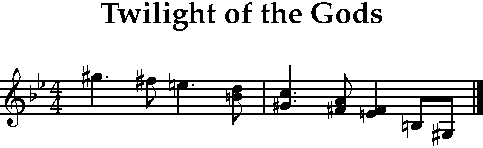
\includegraphics{music/twilight-crop.pdf}
        \caption{诸神的黄昏主导动机\cite{wagner1876gotterdammerung}}
        \label{fig:twilight}
      \end{figure}
      
      社会存在决定社会意识,因此,瓦格纳歌剧艺术中存在着很多当时社会存在的元素,
      例如图~\ref{fig:hagen} 是哈根(Hagen)的主导动机,
      其中充满了冷酷和无情,正是当时充满阴谋邪恶的一个缩影。
      \begin{figure}[htbp]
        \centering
        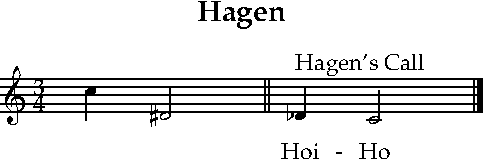
\includegraphics{music/hagen-crop.pdf}
        \caption{哈根的主导动机\cite{wagner1876gotterdammerung}}
        \label{fig:hagen}
      \end{figure}

      但是,瓦格纳歌剧作为一个好的社会意识,并没有止步于反映社会存在,
      而是进一步给出了他的新社会——最终的净化。
      《诸神的黄昏》中的大火没有白烧,
      智慧、并且善解人意的女武神布伦希尔德(Br\"unnhilde)最后的绝唱中,
      她总结道英雄齐格弗里德必然要背叛她,
      命运也必然如此走向最后的毁灭。
      不过大火燃尽了世界的罪恶,
      罪恶的源泉``尼伯龙根的指环''也被重新熔为莱茵的黄金,
      世界得到了净化,布伦希尔德自己也获得了救赎。
      \begin{figure}[htbp]
        \centering
        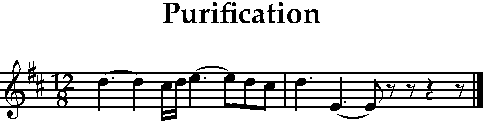
\includegraphics[width=\linewidth]{music/purification-crop.pdf}
        \caption{净化的主导动机\cite{wagner1876gotterdammerung}}
      \end{figure}

      1992版拜罗伊特制作巴伦博伊姆指挥的《诸神的黄昏》特别令我感动,
      当火焰燃遍世界之后,世界重新开始,一个男孩走向了女孩将她牵起,
      不说我们却都知道他们就是齐格弗里德和布伦希尔德!
      这是最具有希望的一个版本,重生之后我们又看到了光明。

      那么这最后的光明是什么呢?瓦格纳没有完全给出,而是给了我们思考的空间。
      ``社会意识对社会存在具有能动的反作用''\cite{book},
      引发深思之后,实践会将这些理念转化为现实。


    \subsection{爱情与救赎}

      世界新秩序之上是永恒的``爱情与救赎''的思考。
      爱情与救赎之前是遗忘,图~\ref{fig:amnesia} 给出了《诸神的黄昏》中的
      遗忘动机。
      \begin{figure}[htbp]
        \centering
        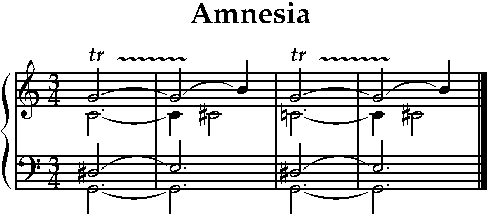
\includegraphics{music/amnesia-crop.pdf}
        \caption{遗忘的主导动机\cite{wagner1876gotterdammerung}}
        \label{fig:amnesia}
      \end{figure}

      为什么爱情与救赎在世界新秩序之上呢?
      这是因为爱情与救赎在``遗忘''的对立面,
      提出了个人、国家、世界所有层面上的新秩序。
      当个人命运与国家、世界绑定时,
      爱情或个人的救赎在一定程度上就是具有对于社会的最大意义;
      另一方面,国家世界都需要个人做好自己的那一部分工作。
      从源头上,西方的基督教文化社会存在中圣经(Holy Bible)
      对原罪和救赎的探讨已经深入人心,
      因此,作品中表现的爱情与救赎是基于其社会存在的。

      《特里斯坦与伊索尔德》(Tristan und Isolde, 1859)
      最后的爱之死(Liebestod)令人感动,是对自由的争取,
      与传统的决裂,纵使其形式是死亡。
      这就是社会意识在反作用推动社会存在。
      现如今,人们大都可以寻找自己的爱情,
      是社会的进步,其中这样的艺术作品对于改变人们的观念功不可没。
      图~\ref{fig:love} 给出了《诸神的黄昏》布伦希尔德和齐格弗里德之爱的主导动机。
      \begin{figure}[htbp]
        \centering
        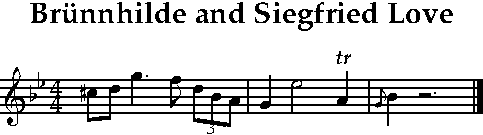
\includegraphics[width=\linewidth]{music/love-crop.pdf}
        \caption{爱情的主导动机\cite{wagner1876gotterdammerung}}
        \label{fig:love}
      \end{figure}

      《帕西法尔》(Parsifal, 1882)则从救赎上对人们进行引导,
      是构建未来社会的必要。
      因此,当新世界秩序的构建凝结在``爱情与救赎''这个话题上,
      艺术更体现出了其``教育''作用,即``社会意识''对``社会存在''的反作用。
      所以,瓦格纳说在完美社会中不需要艺术。
      而在现在我们无法达到终极的完美社会的时候,艺术为我们指明了一条奋斗的路线。

  \section{瓦格纳歌剧的现代意义}

    瓦格纳歌剧仍然具有很强的现代意义,主要体现在下面的两个方面:
    \begin{itemize}
      \item 瓦格纳歌剧仍然作为德国民族认同和团结的媒介。瓦格纳歌剧传达的国家层面价值仍然发挥着作用,它美妙的音乐也使得其成为德国文化乃至世界文化不可或缺的部分;
      \item 瓦格纳歌剧可以被很好地重新诠释以适应最新的社会存在。歌剧虽然音乐台词已定,其制作都可以重新设计,以使得艺术传达出最符合社会存在需求的效果。
    \end{itemize}
    将瓦格纳歌剧与中国国情紧密结合将会制作出深刻、服务社会发展的艺术作品,属于人民的艺术,
    而不是高高在上不可触及的。

  \section{总结}

    瓦格纳歌剧是艺术表现形式的一大代表,
    作为社会意识决定于社会存在,又反作用于社会存在,同时具有相对独立性等辩证关系。
    从瓦格纳歌剧的四重境界出发,报告结合音乐细节分析了这些辩证关系,
    并指出了其现代意义。

  \appendix

  \section{乐谱代码}

    论文中乐谱代码使用 \LaTeX{} 中的工具 M-TX,其代码如下:

    \lstinputlisting{music/hero.mtx}
    \lstinputlisting{music/twilight.mtx}
    \lstinputlisting{music/hagen.mtx}
    \lstinputlisting{music/purification.mtx}
    \lstinputlisting{music/amnesia.mtx}
    \lstinputlisting{music/love.mtx}
    % \lstinputlisting{music/bruennhilde.mtx}
    % \lstinputlisting{music/bloodbro.mtx}
    % \lstinputlisting{music/revenge.mtx}

  \printbibliography[title={参考文献}]

\end{document}